
In this section, we discuss the structure of the VDF after a long simulation
period (60 wave periods for 1 AU and 45 periods for 0.3 AU). In the case of 1 AU
parameters, the following figures will include the core, halo, strahl, and 
total distribution function, while in 0.3 AU parameters, the distribution 
includes only the core and strahl electrons. In this non-relativistic range of 
energy, the $R$ surfaces are almost straight lines, so only the 
intersections (white crosses) with the $v_\perp=0$ axis are plotted to signify 
their locations (as derived in
\cref{eq:resonant_velocity}). The concentric ellipses (black curves) are the
constant $H$ surfaces (from \cref{eq:constant_H_surface}), the center of which is the Landau resonance $(n=0)$. The intersections of the $H$ surfaces with the
$v_\perp=0$ axis show the $n=\pm1,\pm2,...$ radially from the $n=0$ mode. Recall
that in this work's convention, the $n<0$ modes are always along the parallel 
velocity range and the $n>0$ modes are along the anti-parallel range (as 
opposed to most papers in the literature).

\subsection{Single whistlers at 1 AU}
\begin{figure}
    \centering
    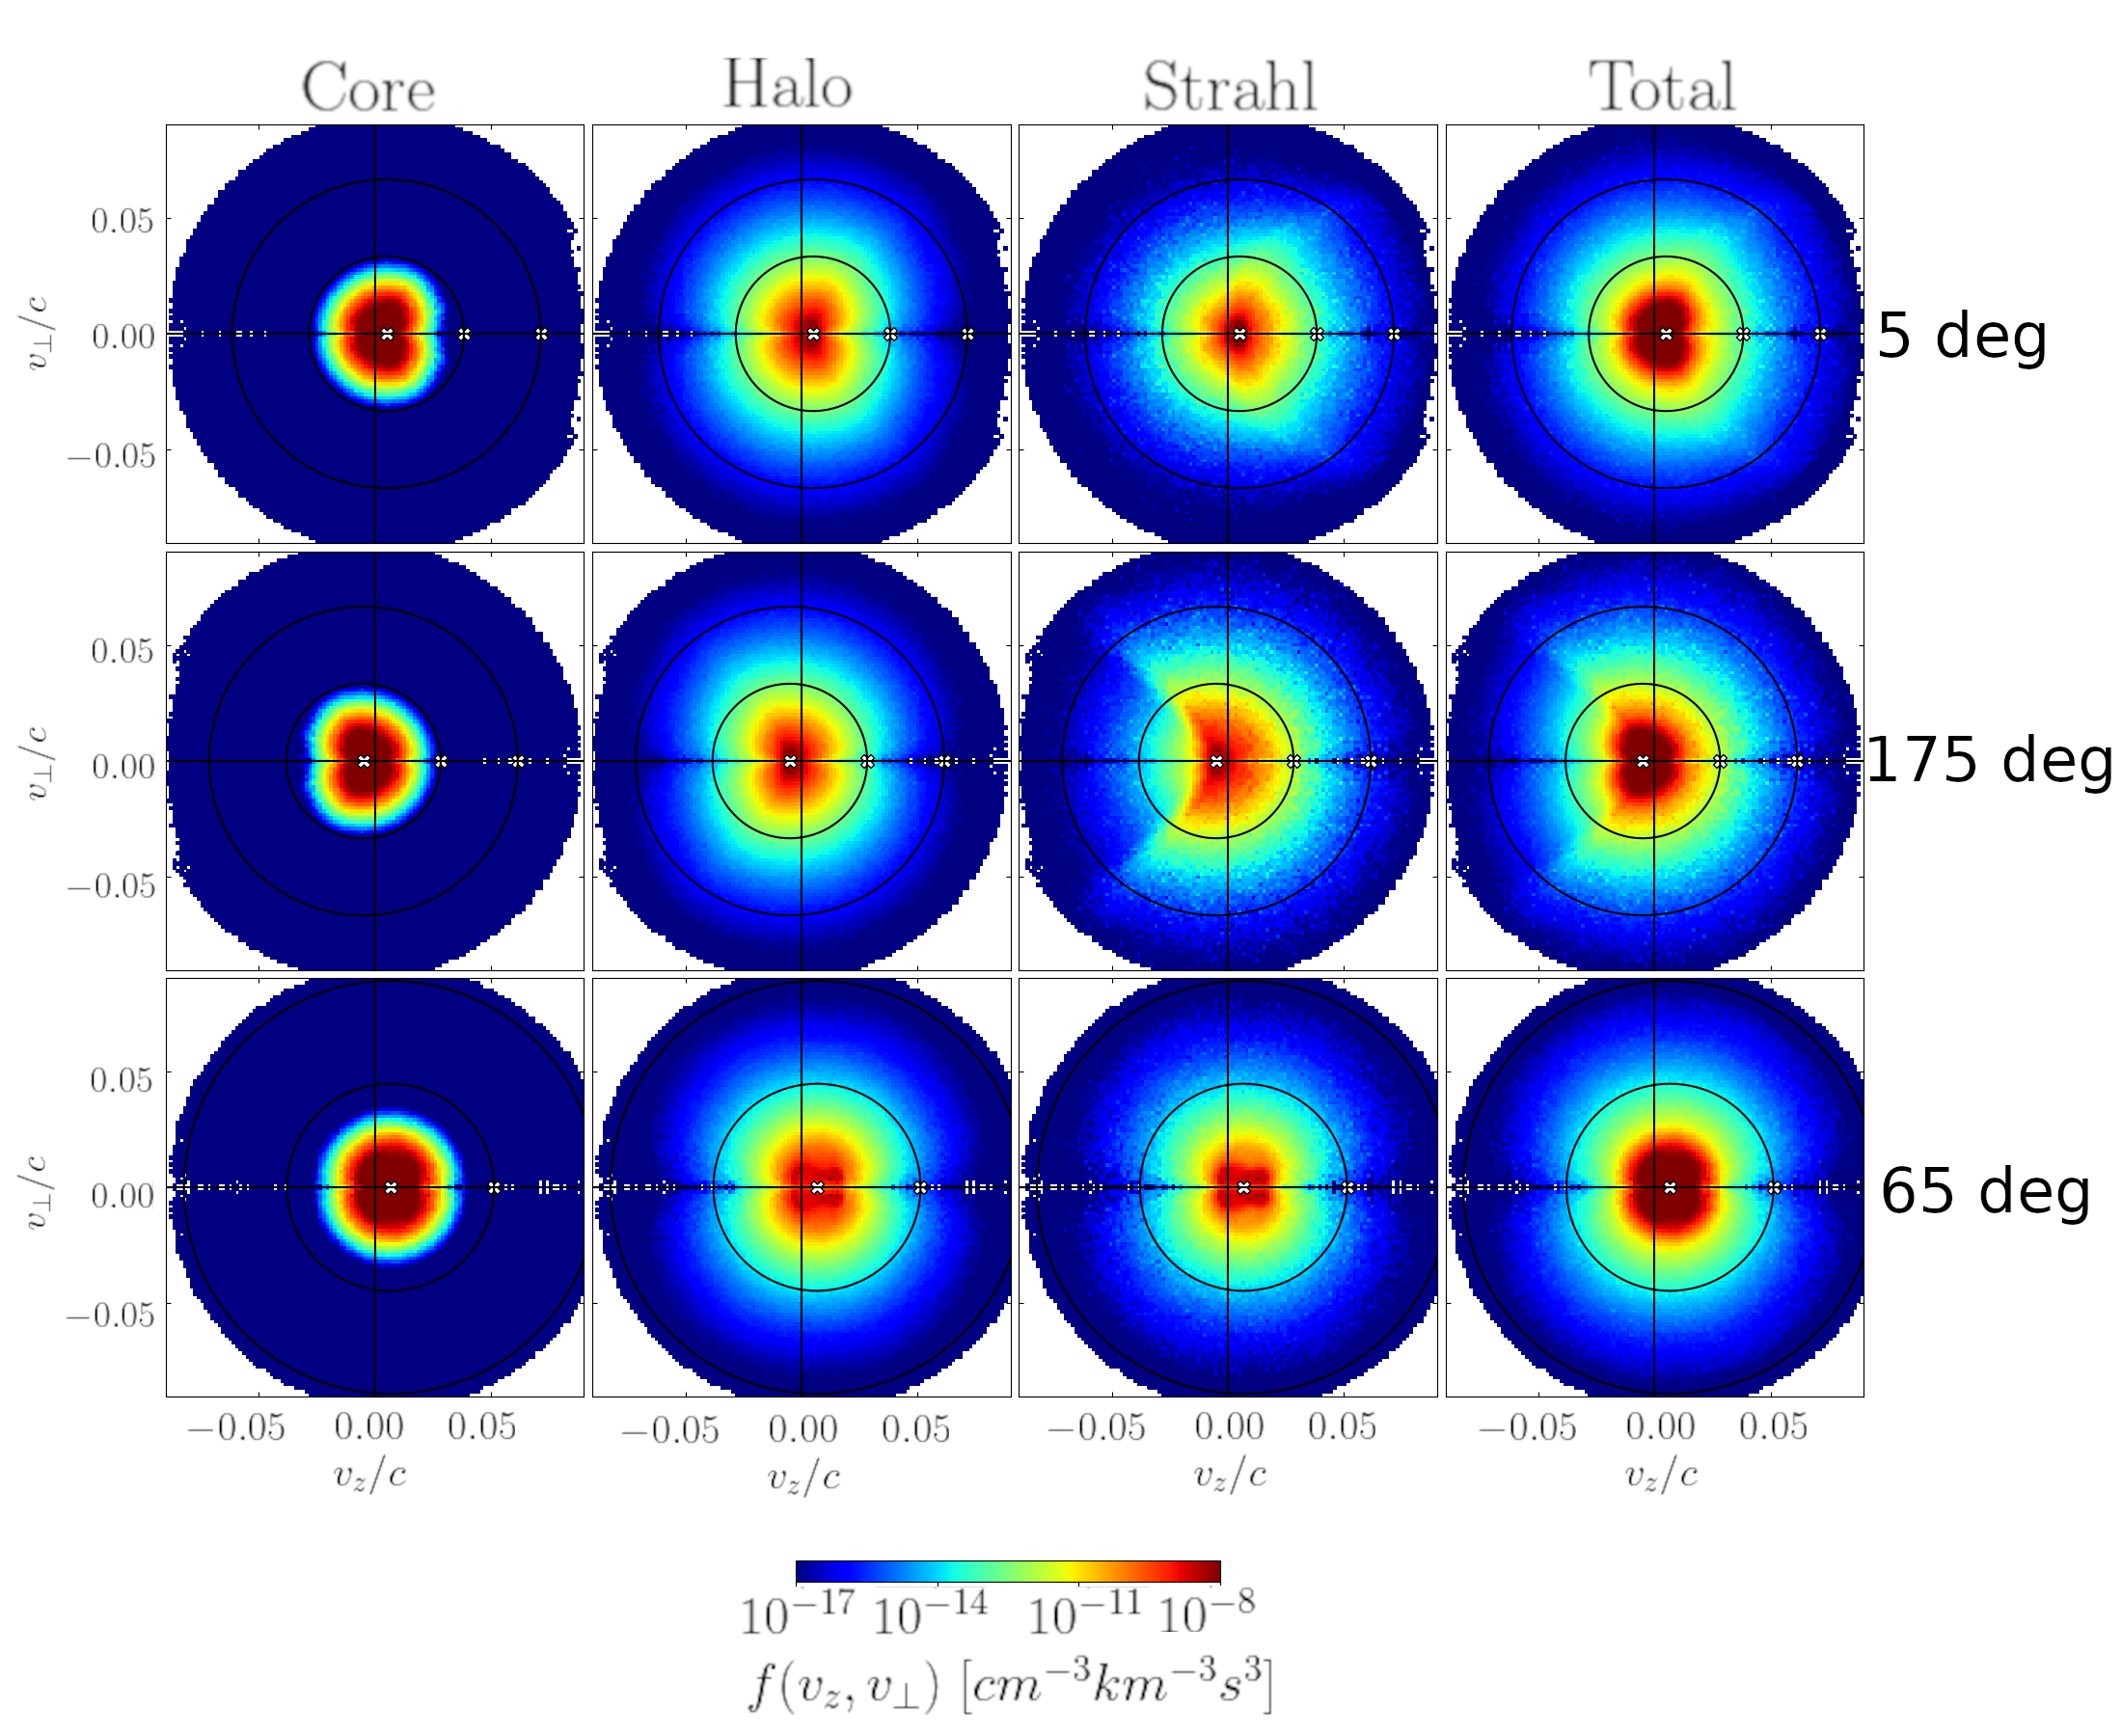
\includegraphics[width=\textwidth]{single_whistlers_1AU.png}
    \caption{VDF of electron populations after 60 wave periods of interaction
    with a single whistler at 1 AU. From top to bottom, the rows are the
simulations with the $5^\circ$, $175^\circ$, and $65^\circ$ wave.}
    \label{fig:single_whistlers_1AU}
\end{figure}

For single whistlers, \cref{fig:single_whistlers_1AU} shows the results from 
three simulations which demonstrate the interactions with (from
top to bottom) an almost parallel ($5^\circ$), an almost antiparallel
($175^\circ$), and an oblique ($65^\circ$) wave after 60 wave periods. The
final VDF of the two parallel cases approximately mirror each other, however,
the structures are not entirely identical since the background field points
along the wave in one case and against the wave in another, while the strahl
electrons are propagating along the field. The first two rows
indicate that parallel waves are able to scatter electrons to a certain extent.
However, there is a prominent bow-like feature near the $n=-1$ mode at an angle
of $\sim50^\circ$ around the $v_\perp=0$ axis, which is most apparent for the
anti-parallel case. The last row indicates that the interaction with an oblique
whistler efficiently isotropizes the strahl, which results in a structure
almost identical to the halo by the end of the simulation period. However, there
is a lack of high energy and parallel propagating particles, which has been
observed in the energy-pitch angle distribution in PSP data
\citep{Cattell2021b}. This makes the final results not completely isotropic.
Thus, it is not suitable to apply the fitting procedure for the model
defined in \cref{eq:kappa} that \cite{Wilson2019} used for satellite observations of the VDF.

To better understand the VDF structures, the
trajectories of a few particles interacting with the 5$^\circ$ and
65$^\circ$ waves during the entire simulation period are shown in \cref{fig:single_O5_1_AU}. In panels A1, B1, C1, and D1, the particles move along their corresponding $H$
surfaces as expected. The corresponding histograms (A2, B2, C2, and D2) show the
points along the particle's trajectory where they hover around the most. In the
interaction with the 5$^\circ$ wave (panels A and B), the histograms are uniform, indicating that the particles bounce back and forth in a quasi-periodic motion. There is a point of ``reflection'' for each energy, which results in the bow-like feature in the VDF. These points are close to the intersections of the $H$ surfaces and the $n<0$ resonances. This can be due to a combined effect of (a) magnetic mirroring due to the large wave fields comparable to the ambient field and (b) resonant interaction. Effect (a) is a speculation that needs further analysis beyond the scope of this thesis. Here we shall only offer an explanation for (b) from the theory of resonance derived in \cref{sec:theory}.

For $n<0$, the electron overtakes the wave when it observes a left-hand polarized electromagnetic field in its own frame. Thus, being a right-hand particle, it no longer interacts resonantly. This results in the deceleration of $v_z$ to the negative range where resonant interaction is enabled once again because the particle observes a right-hand polarized wave. It would be interesting to study whether this occurs for a self-consistently simulated wave-particle interaction using PIC code. This is because the $n<0$ modes are usually where the particle transfers its energy to the wave as it rotates out of phase with the fields, leading to wave generation instead of damping \citep{Tsurutani1997}. Thus, the wave is modified due to this type of quasi-parallel whistler heat-flux instability \citep{RobergClark2019,Micera2020} and both the $H$ and $R$ surfaces are altered accordingly. This might allow the VDF to become more isotropic for particles under interactions with parallel whistlers.

\begin{figure}[hbtp]
    \centering
    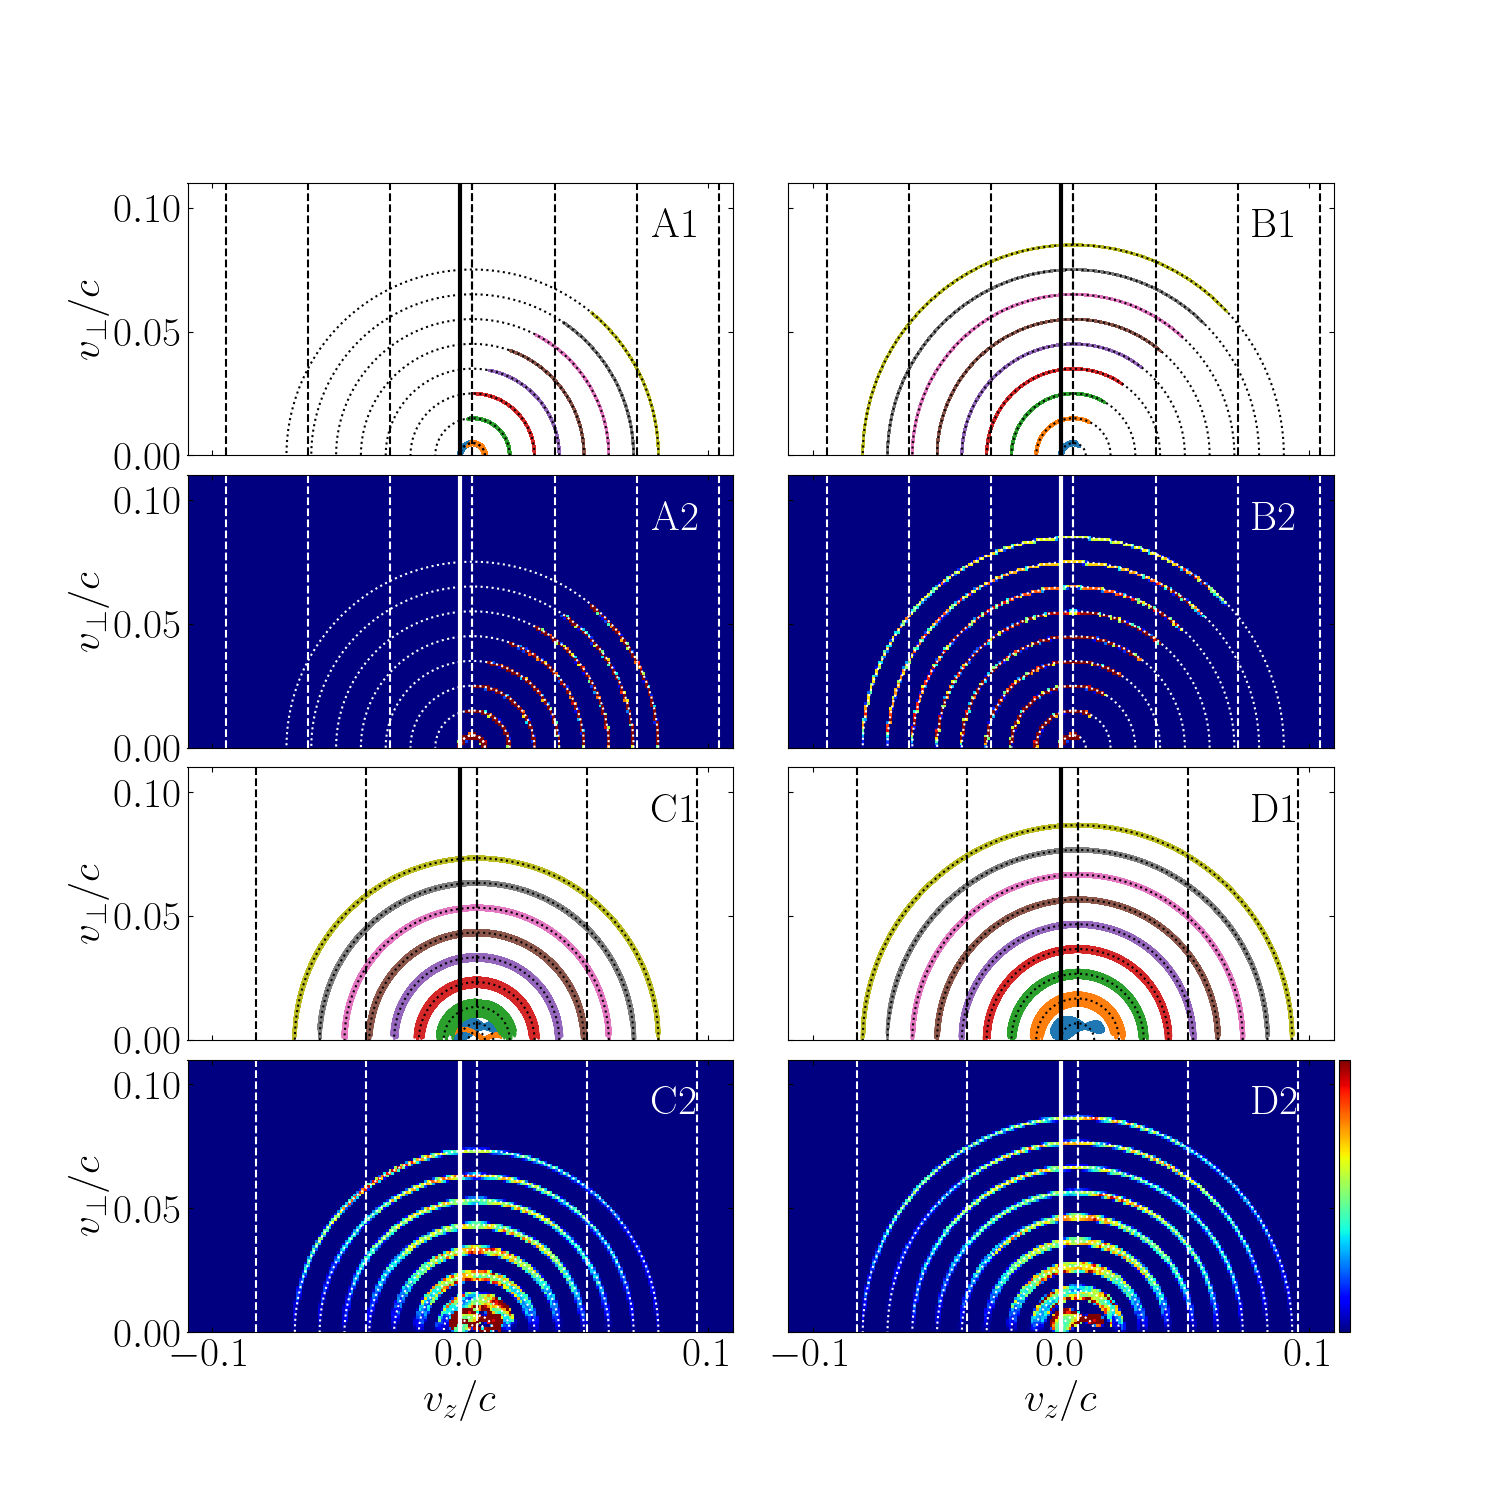
\includegraphics[width=\textwidth]{single_combo_trajectory.png}
    \caption{Traces of electron trajectories in the entire simulation period
        (1 AU parameters) and
        their corresponding histograms. The panels show those for electrons that are originally parallel (A1-A2) and antiparallel (B1-B2) to the
        single 5$^\circ$ whistler. Similarly, (C1-C2) and (D1-D2) are those
        parallel and antiparallel to the single 65$^\circ$ whistler. Their
    initial speeds are $0,0.01,0.02,...,0.08c$, which correspond to
$0,26,102,...1643$\,\si{eV}. The dotted curves are the constant $H$ ellipses
corresponding to the particle's intitial energy, while the dashed straight lines
are the $R$ surfaces corresponding to (from left to right) $n=3,2,...,-3$. The
solid lines are the $v_z=0$ axis.}
        \label{fig:single_O5_1_AU}
\end{figure}

Because the polarization for an oblique wave is elliptical, it is a
combination of both right-hand and left-hand waves. This allows for anomalous
interactions to occur, which happens when an electron (right-hand) interacts
with the $n>0$ harmonics of a left-hand wave by overtaking it
and observing a right-hand polarized electromagnetic field
\citep{Tsurutani1997}. Consequently, the scattering of electrons is more
isotropic in panels C and D, where both parallel and anti-parallel particles behave similarly.

\begin{figure}
    \centering
    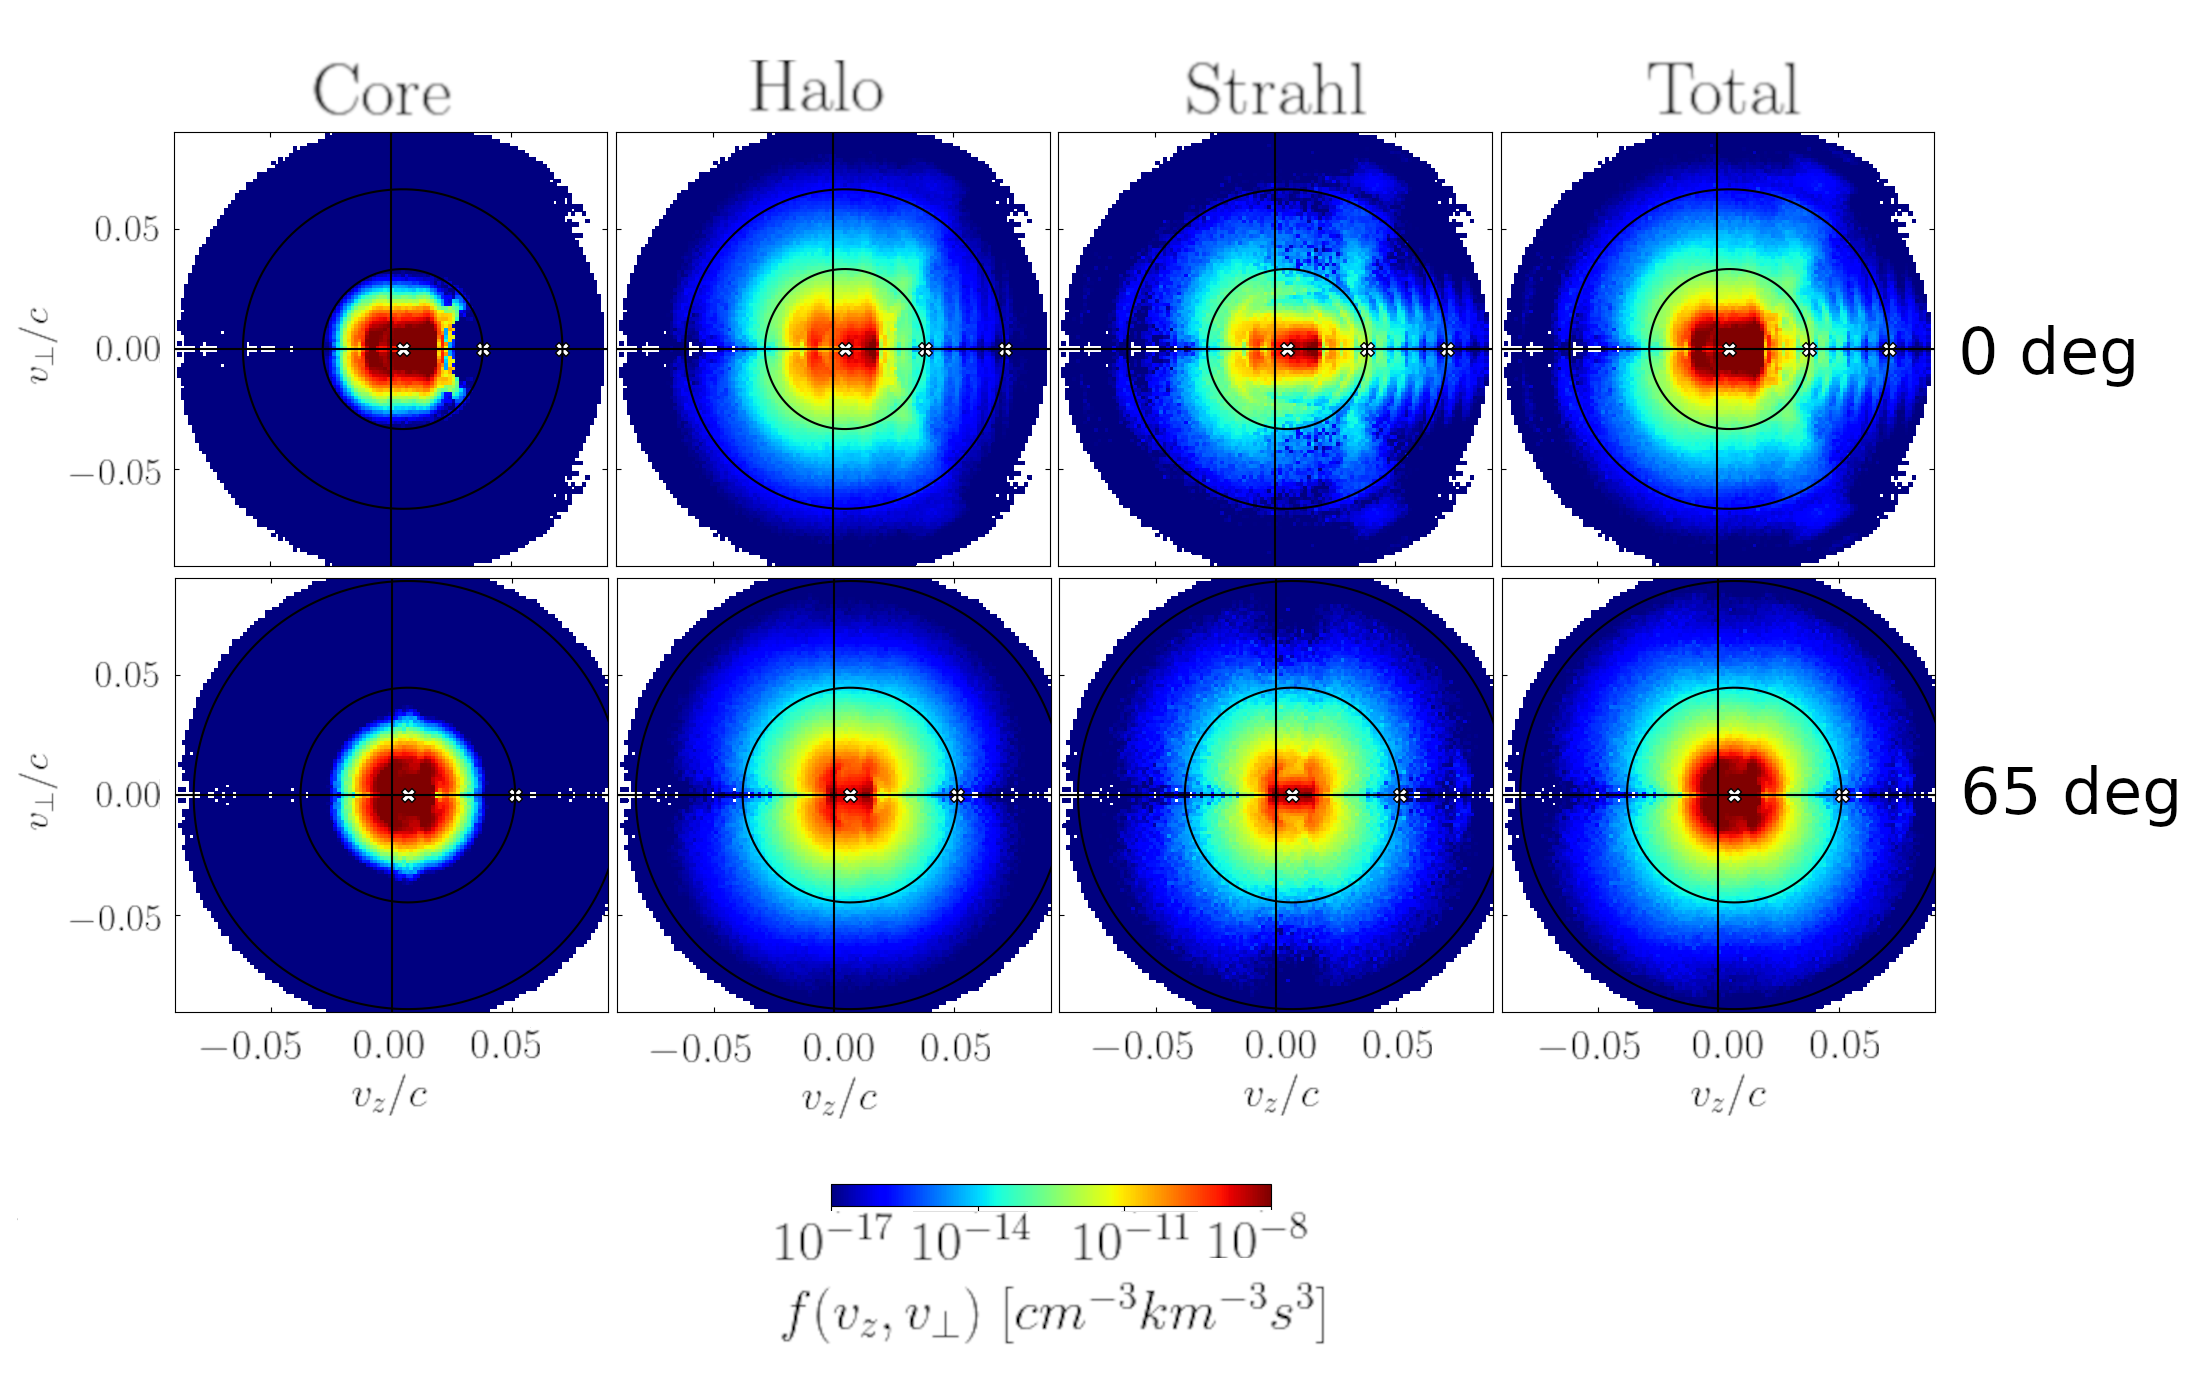
\includegraphics[width=\textwidth]{whistler_packets_1AU.png}
    \caption{VDF of electron populations after 60 wave periods of interaction
        with a $0^\circ$ (top row) and 65$^\circ$ (bottom row) whistler packet at 1 AU.}
\label{fig:whistler_packets_1AU}
\end{figure}

\subsection{Whistler packets at 1 AU}


\cref{fig:whistler_packets_1AU} shows the final VDF after 60 wave periods of
interaction with a $0^\circ$ packet and a $65^\circ$ packet in 1 AU parameters. A region of particle loss similar to that in the single wave parallel whistlers in the previous section can be seen in the $0^\circ$ packet. However, in addition to the bow-like region, there is also a vertical structure near the $n=-1$ harmonic. Because multiple frequencies are contained in the packet, the $R$ surfaces are now clustered. \cref{fig:packet_O0_1_AU} shows the surfaces corresponding to the packet's mean frequency wave. In panel B2, there are electrons trapped around the $n=-1$ cluster of $R$ surfaces. Those particles are energetic enough to enter the envelope of the cluster but they cannot escape, resulting in this vertical structure in the VDF. This further supports the explanation from the theory of resonance. In the frame of the mean-frequency
wave, there are other waves of different frequencies, which move in both
directions with respect to it. Their combined effects cause the trapping
around $n=-1$. However, large amplitude waves at $0^\circ$ are not seen in
the solar wind at 1 AU. The large amplitude waves at 1 AU are oblique, like the
$65^\circ$ packet. For this case, the electron interaction with the packet
is similar to the case of a single whistler for the strahl.

\begin{figure}[hbtp]
    \centering
    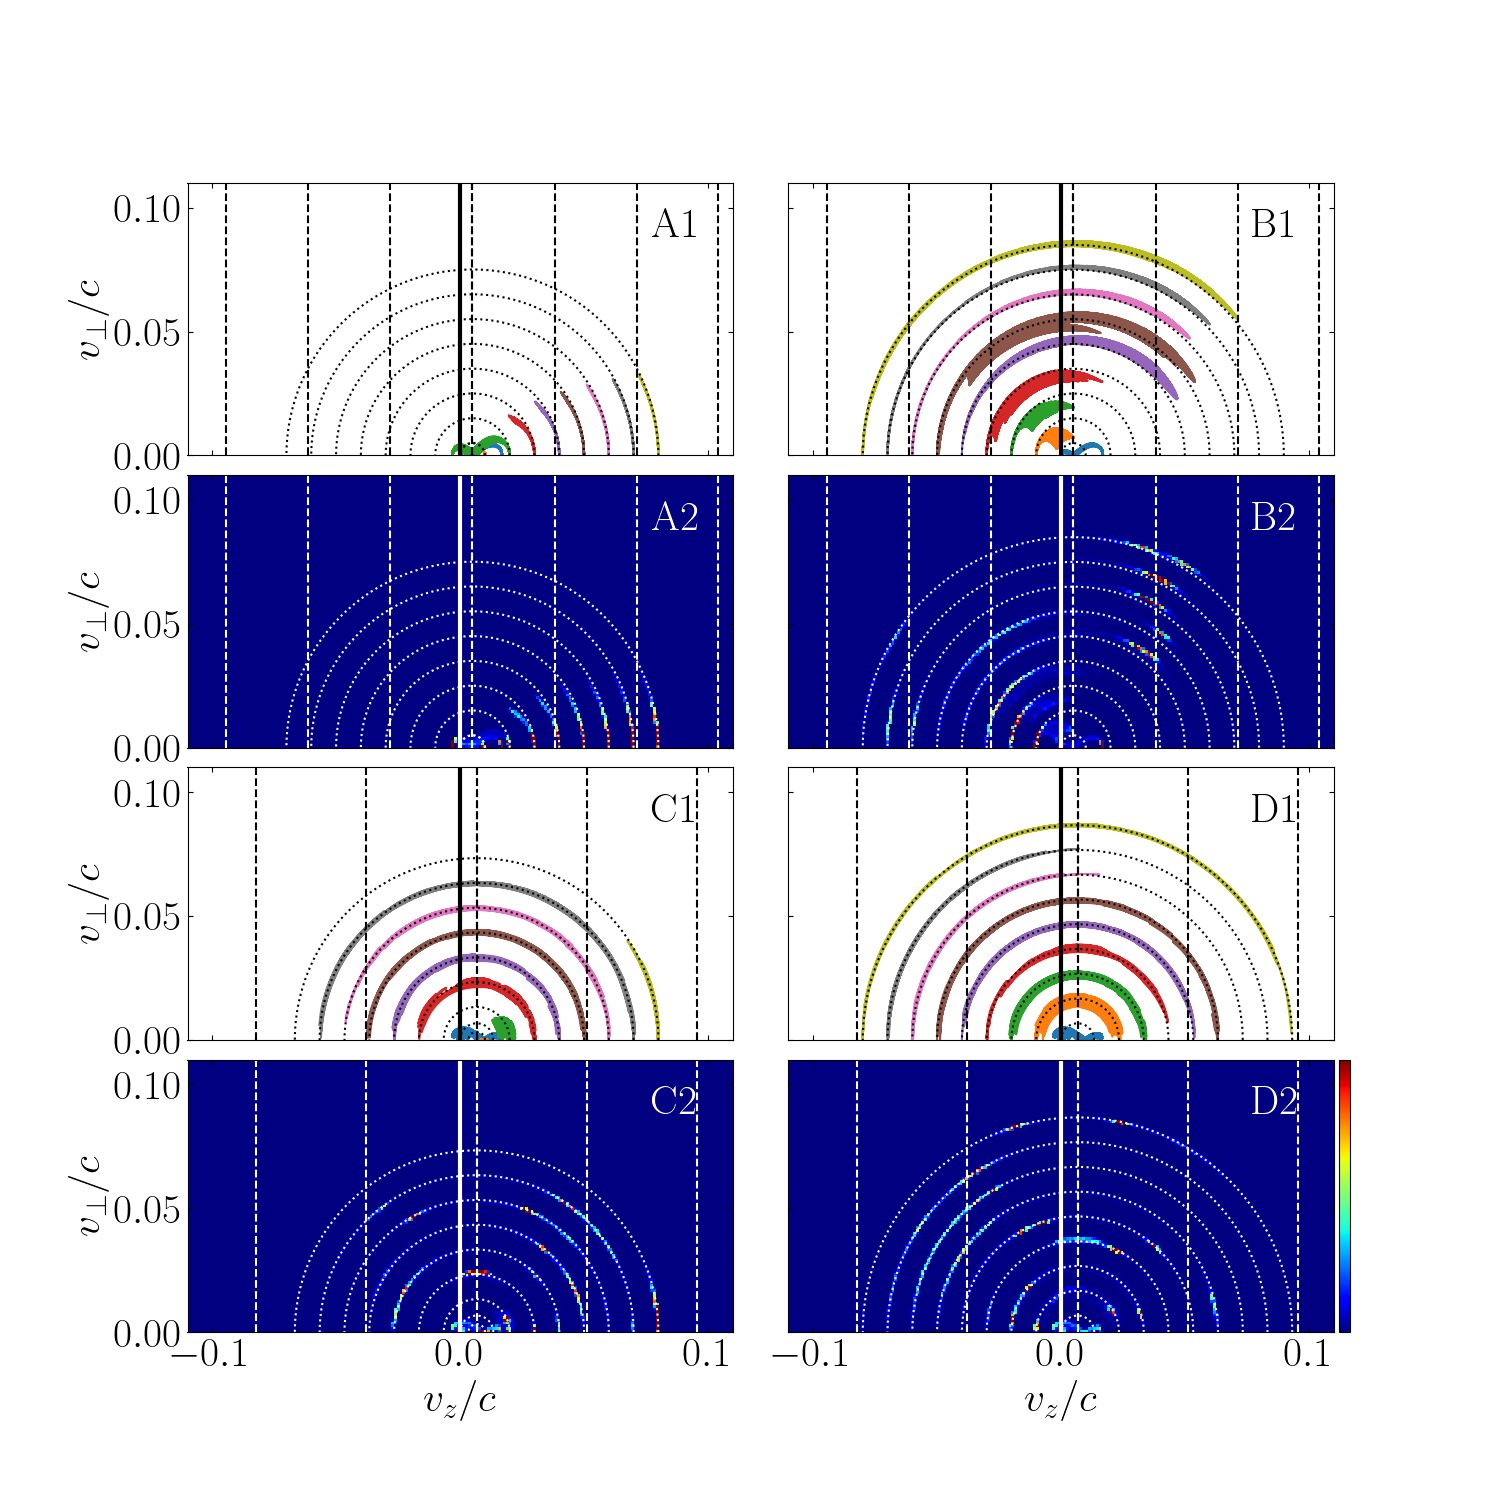
\includegraphics[width=\textwidth]{packet_combo_trajectory.png}
    \caption{Traces of electron trajectories in the entire simulation period
        (1 AU parameters) and their corresponding histograms. The panels are
        similar to those in \cref{fig:single_O5_1_AU}, but the electrons are
        under interactions with a 0$^\circ$ packet (A and B) and a 65$^\circ$
        packet (C and D).}
    \label{fig:packet_O0_1_AU}
\end{figure}

The scattering of particles interacting with the oblique packet is highly
localized and often in between the resonances (see panels C2 and D2). This is
most likely due to the overlapping resonance widths associated with each mode
\citep{Karimabadi1990}. In this work, the single-wave resonance surfaces are
spaced fairly closely between each harmonic $n$. The overlap of resonance widths
can cause more nonlinear and complicated interactions to occur. The calculation
of the widths is beyond the scope of this thesis.

\subsection{Whistler packets at 0.3 AU}

\begin{figure}[hbtp]
    \centering
    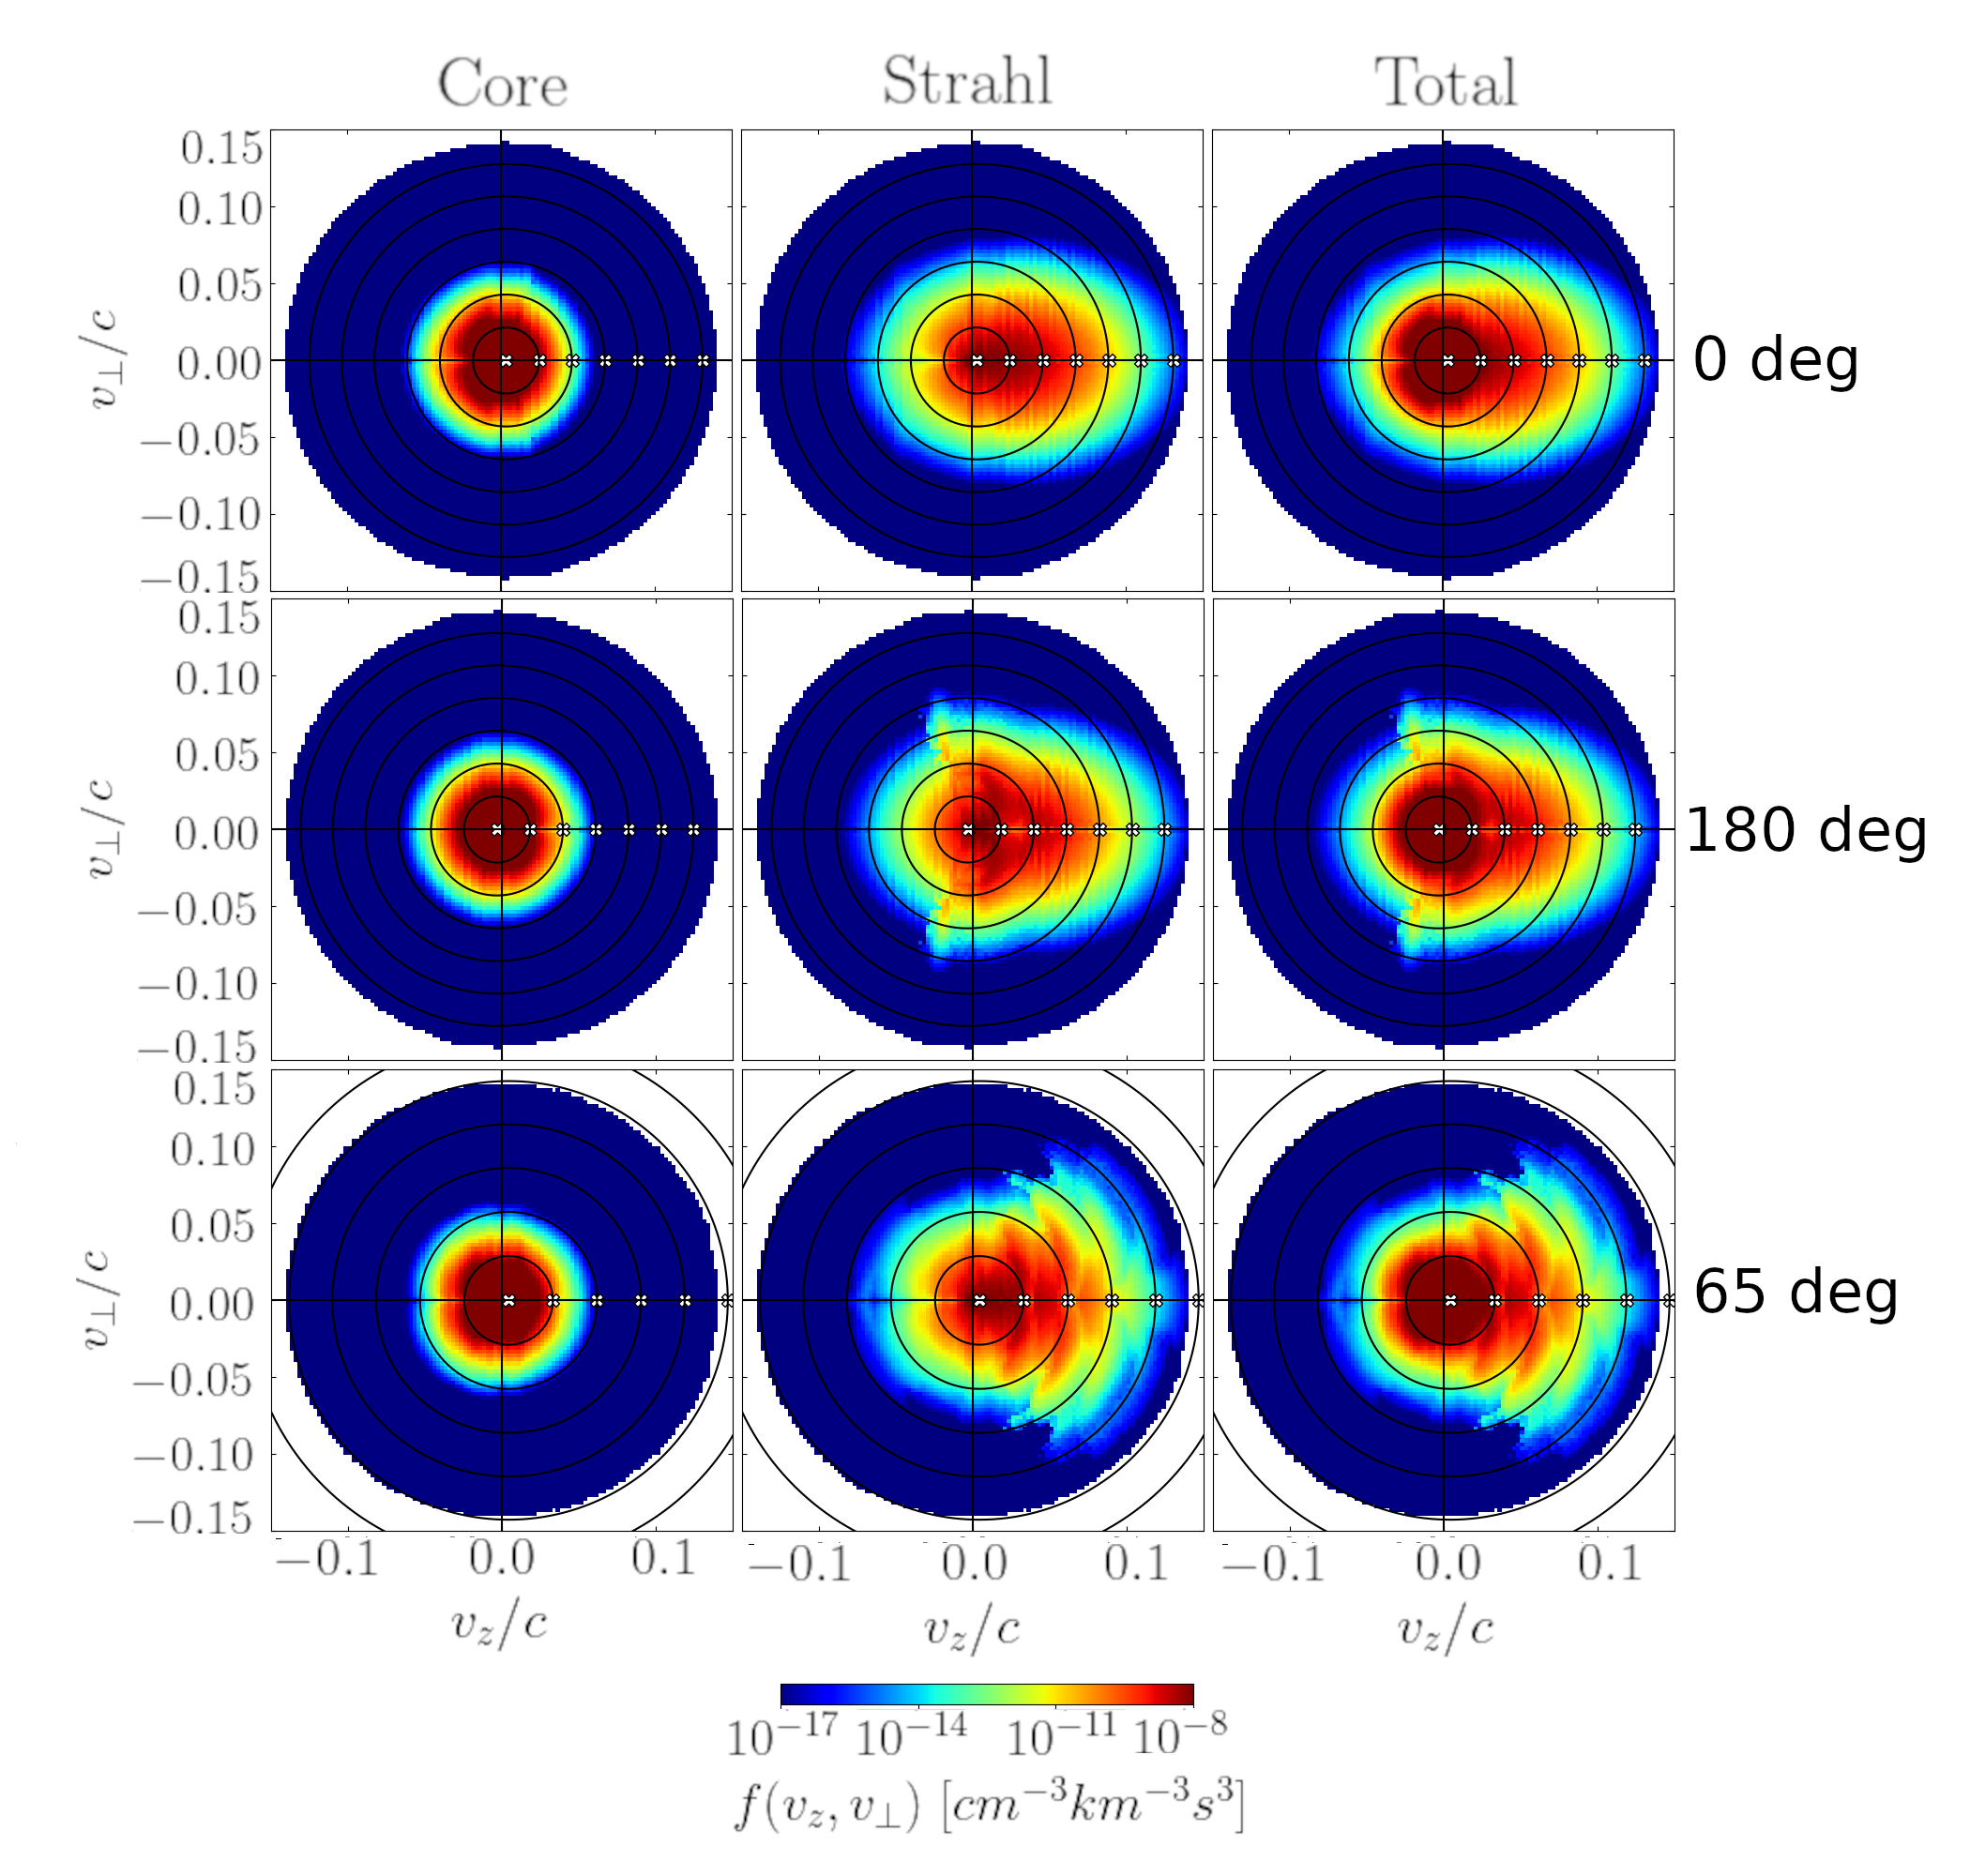
\includegraphics[width=\textwidth]{whistler_packets_03AU.png}
    \caption{VDF of electron populations after 45 wave periods of interaction
    with whistler packets at 0.3 AU. From top to bottom, the rows are the
simulations with the $0^\circ$, $180^\circ$, and $65^\circ$ wave.}
\label{fig:whistler_packets_03AU}
\end{figure}

For interactions with whistler packets in 0.3 AU parameters, we observe the
formation of ``horn''-like features in the VDF at the locations of the
$R$ intersections in the case of oblique propagation (see
\cref{fig:whistler_packets_03AU}). This is similar to what was reported in
\cite{RobergClark2019}. However, they studied very relativistic
electrons, which resulted in more defined horn features as the particle velocity
term dominates in the canonical momentum. In the discussed parameters, this 
dominance is weaker, which results in broader horns. Parallel packets do not 
scatter the strahl as efficiently as oblique packets near the Sun,
as similar to the discussion in \cite{Vocks2005}. \cite{Halekas2020b} reported
that the heat flux observed at 0.3 AU was consistent with the threshold for
oblique whistler fan instability. So these results are consistent with near-Sun 
observations.



